\documentclass[a4paper,11pt]{article}

%% packages

\usepackage{blindtext} % needed for creating dummy text passages
%\usepackage{ngerman} % needed for German default language
\usepackage{amsmath} % needed for command eqref
\usepackage{amssymb} % needed for math fonts
\usepackage[colorlinks=true,breaklinks]{hyperref} % needed for creating hyperlinks in the document, the option colorlinks=true gets rid of the awful boxes, breaklinks breaks lonkg links (list of figures), and ngerman sets everything for german as default hyperlinks language
\usepackage[hyphenbreaks]{breakurl} % ben�tigt f�r das Brechen von URLs in Literaturreferenzen, hyphenbreaks auch bei links, die �ber eine Seite gehen (mit hyphenation).
\usepackage{xcolor}
\definecolor{c1}{rgb}{0,0,1} % blue
\definecolor{c2}{rgb}{0,0.3,0.9} % light blue
\definecolor{c3}{rgb}{0.3,0,0.9} % red blue
\hypersetup{
    linkcolor={c1}, % internal links
    citecolor={c2}, % citations
    urlcolor={c3} % external links/urls
}
%\usepackage{cite} % needed for cite
\usepackage[square,authoryear]{natbib} % needed for cite and abbrvnat bibliography style
\usepackage[nottoc]{tocbibind} % needed for displaying bibliography and other in the table of contents
\usepackage{graphicx} % needed for \includegraphics 
\usepackage{longtable} % needed for long tables over pages
\usepackage{bigstrut} % needed for the command \bigstrut
\usepackage{enumerate} % needed for some options in enumerate
%\usepackage{todonotes} % needed for todos
\usepackage{makeidx} % needed for creating an index
\makeindex
\usepackage{gensymb}
\usepackage{url}

%% page settings

\usepackage[top=5mm, bottom=5mm,left=15mm,right=15mm]{geometry} % needed for page border settings
\parindent=0mm % for space of first line of new text block
\sloppy % for writing with hyphenless justification (tries to)
\hyphenation{} % use hyphenation of tolerance parametershttp://www.jr-x.de/publikationen/latex/tipps/zeilenumbruch.html
\hyphenpenalty=10000
\exhyphenpenalty=10000
\usepackage{fancyhdr} % needed for head and foot options
%% my macros

%% Text fomats
\newcommand{\tbi}[1]{\textbf{\textit{#1}}}

%% Math fonts
\newcommand{\bbA}{\mathbb{A}}
\newcommand{\bbB}{\mathbb{B}}
\newcommand{\bbC}{\mathbb{C}}
\newcommand{\bbD}{\mathbb{D}}
\newcommand{\bbE}{\mathbb{E}}
\newcommand{\bbF}{\mathbb{F}}
\newcommand{\bbG}{\mathbb{G}}
\newcommand{\bbH}{\mathbb{H}}
\newcommand{\bbI}{\mathbb{I}}
\newcommand{\bbJ}{\mathbb{J}}
\newcommand{\bbK}{\mathbb{K}}
\newcommand{\bbL}{\mathbb{L}}
\newcommand{\bbM}{\mathbb{M}}
\newcommand{\bbN}{\mathbb{N}}
\newcommand{\bbO}{\mathbb{O}}
\newcommand{\bbP}{\mathbb{P}}
\newcommand{\bbQ}{\mathbb{Q}}
\newcommand{\bbR}{\mathbb{R}}
\newcommand{\bbS}{\mathbb{S}}
\newcommand{\bbT}{\mathbb{T}}
\newcommand{\bbU}{\mathbb{U}}
\newcommand{\bbV}{\mathbb{V}}
\newcommand{\bbW}{\mathbb{W}}
\newcommand{\bbX}{\mathbb{X}}
\newcommand{\bbY}{\mathbb{Y}}
\newcommand{\bbZ}{\mathbb{Z}}
\usepackage{subfigure}

\begin{document}
	Thalagala B.P. 180631J
\begin{center}	
{	\Large\textbf{In-class assignment 1}}\\[2mm]	

\textbf{October 27, 2021}
\end{center}

\subsection*{1. ARQ protocol to improve the reliability of data transmission}
Error control is one of the main functions in the Datalink layer in OSI model which improves the reliability of data transmission. It consists of Error detection and Error correction schemes. Error correction can be further classified in to two categories as \textit{Forward Error Correction} and \textit{Feedback Error Control}. Go-back-N and Selective re-transmission ARQs(Automatic repeat requests) come under the Feedback Error Control scheme. 

\begin{figure}[!h]
	\centering
	\subfigure[Go-back-N]
	{ 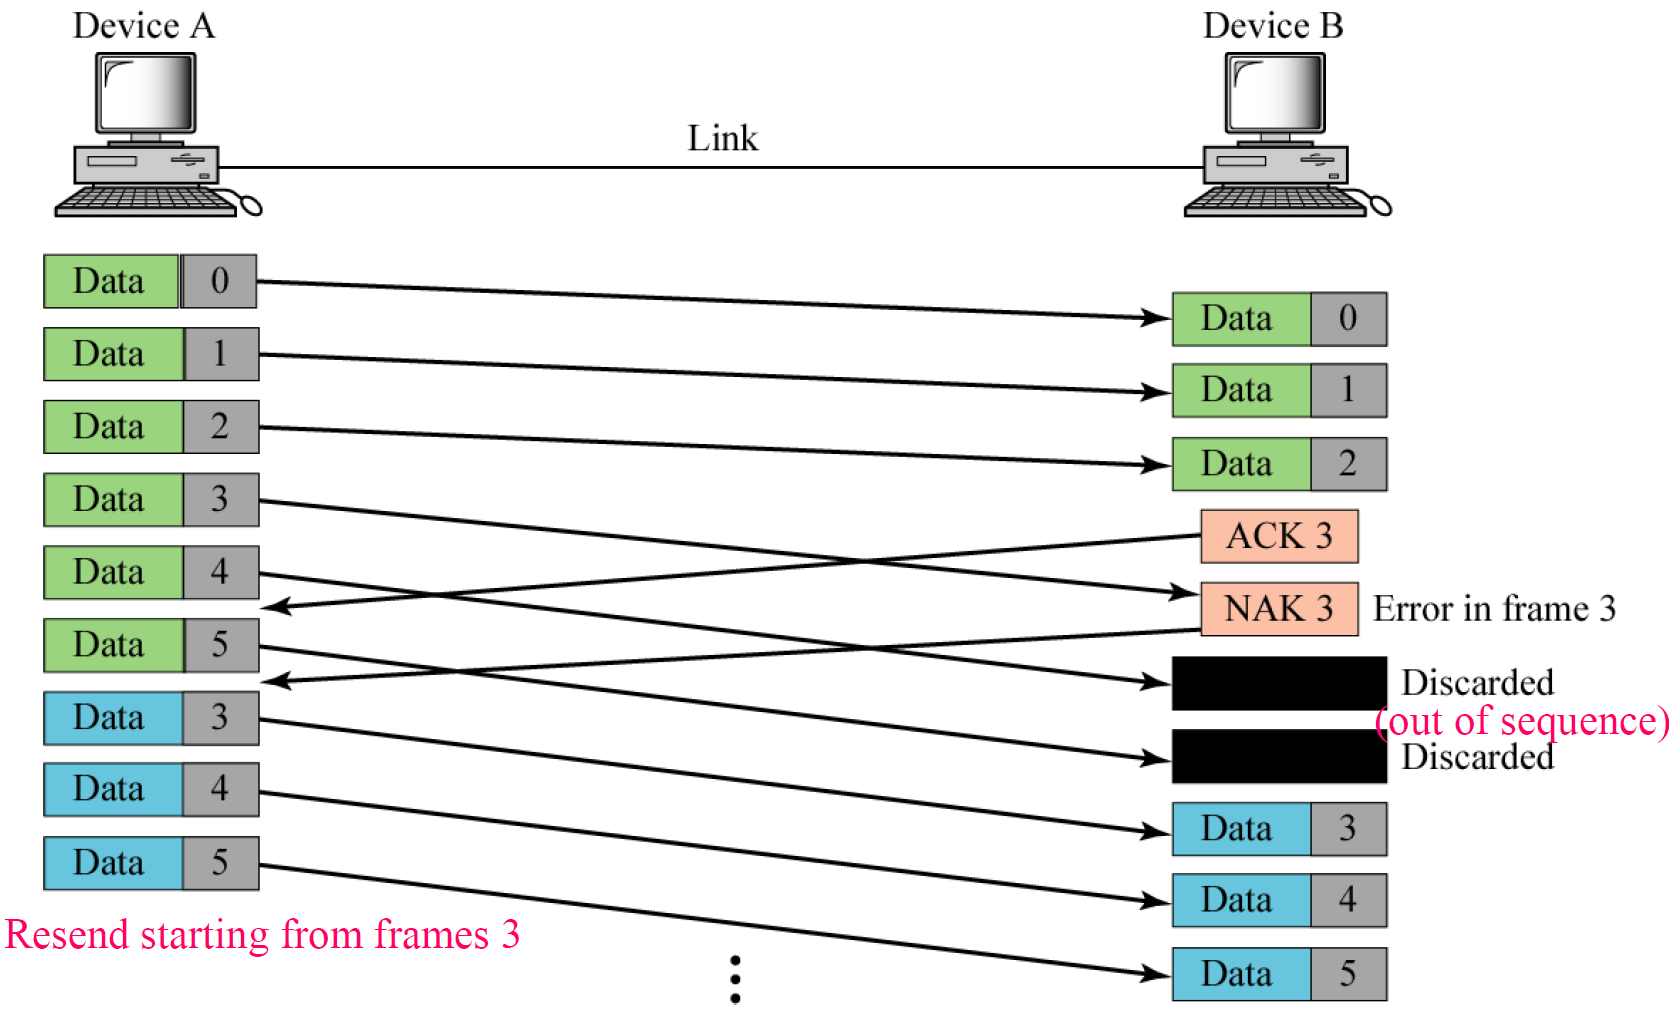
\includegraphics[scale=0.27]{figures/gbn}
	}\hfill
	\subfigure[Selective re-transmission]
	{ 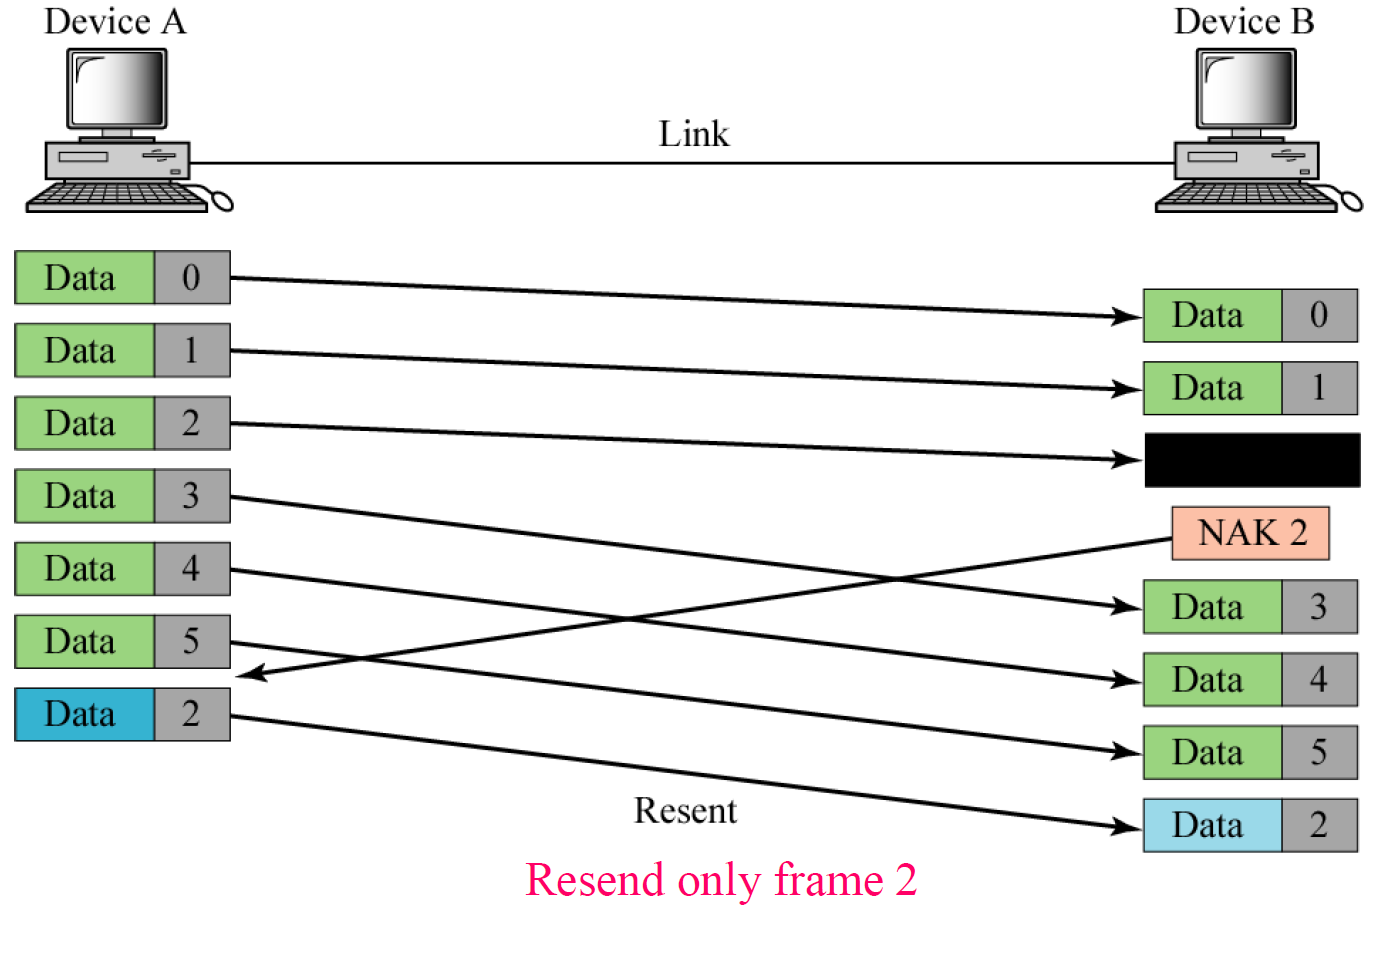
\includegraphics[scale=0.27]{figures/srj}
	}
\end{figure}

\paragraph{Go-back-N ARQ} If the received frame has no error, receiver will send the positive acknowledgment(ACK) to the transmitter specifying the next frame it expects. If the received frame is error-ed, receiver will discard all the upcoming frames and send a negative acknowledgment(NAK) specifying the error-ed frame. Then the transmitter re-transmits the error-ed frame and all the following frames it had sent. 

\paragraph{Selective re-transmission ARQ} In this scheme only the rejected frame will be re-transmitted and receiver accepts the subsequent frames into a buffer without discarding them. This minimizes the number of re-transmissions. However, to keep the subsequent frames receiver has to maintain a sufficient buffer.  

\vfill
\subsection*{2. Expected differences of ARQ protocol between datalink layer and transport layer implementations}

\begin{enumerate}
	
	
	\item Datalink layer's ARQ protocol ensures only the node-to-node(single link - across a wire) error free delivery. Whereas, Transport layer's ARQ protocol ensures the end-to-end delivery of an entire message from source to destination.
	
	\item Implementation differences occur due to the difference between Protocol Data Units (PDUs) of each layer.  Transport Layer's PDU, `\textbf{\textit{segment}}' is much larger than the Datalink Layer's PDU, `\textbf{\textit{frame}}' due to this reason the following differences can be identified.
	
	\begin{enumerate}[~I.]
		\item If an error occurs, re-transmission is efficient with smaller frames (L2 PDU) than larger segments(L4 PDU).
		\item Required buffer size is limited when dealing with frames whereas, larger buffers are required if Selective re-transmission ARQ is implemented in Transport Layer. 
		\item Error detection is efficient with the smaller frames.
		\item Smaller frames prevent, one station occupying the medium for long time. Which then increases the bandwidth utilization.
	\end{enumerate}
	 

	
\end{enumerate}


\end{document}